% declare document class and geometry
%\documentclass[12pt]{article} % use larger type; default would be 10pt
%\usepackage[margin=1in]{geometry} % handle page geometry

% ***********************************************************
% ******************* PHYSICS HEADER ************************
% ***********************************************************
% Version 2
\documentclass[12pt]{article} 





\usepackage{datetime} % allows easy formatting of dates, e.g. \formatdate{dd}{mm}{yyyy}

\usepackage{amsmath} % AMS Math Package
\usepackage{amsthm} % Theorem Formatting
\usepackage{amssymb}	% Math symbols such as \mathbb
\usepackage{graphicx} % Allows for eps images
\usepackage{multicol} % Allows for multiple columns
\usepackage[dvips,letterpaper,margin=1in,bottom=1in]{geometry}
 % Sets margins and page size
\pagestyle{empty} % Removes page numbers
\makeatletter % Need for anything that contains an @ command 
%\renewcommand{\maketitle} % Redefine maketitle to conserve space
%{ \begingroup \vskip 10pt \begin{center} \large {\bf \@title}
%	\vskip 10pt \large \@author \hskip 20pt \@date \end{center}
%  \vskip 10pt \endgroup \setcounter{footnote}{0} }
\makeatother % End of region containing @ commands
\renewcommand{\labelenumi}{(\alph{enumi})} % Use letters for enumerate
% \DeclareMathOperator{\Sample}{Sample}
\let\vaccent=\v % rename builtin command \v{} to \vaccent{}
\renewcommand{\v}[1]{\ensuremath{\mathbf{#1}}} % for vectors
\newcommand{\gv}[1]{\ensuremath{\mbox{\boldmath$ #1 $}}} 
% for vectors of Greek letters
\newcommand{\vx}{\ensuremath{\v{x}}} 
% for vectors of Greek letters
\newcommand{\vy}{\ensuremath{\v{y}}} 
% for vectors of Greek letters
\newcommand{\xdot}{\ensuremath{\dot{x}}} 
% for vectors of Greek letters

\newcommand{\ydot}{\ensuremath{\dot{y}}} 
% for vectors of Greek letters
\usepackage{commath} % for some nice standardized syntax stuff. 
	% \dif, \Dif, \od, \pd, \md, \(abs | envert), \(norm | enVert), \(set | cbr), \sbr, \eval, \int(o | c)(o | c), etc
\newcommand{\bbar}[1]{\bar{\bar{#1}}} % for barring things twice -- use \cbar or \zbar instead of original \bbar

\newcommand{\uv}[1]{\ensuremath{\mathbf{\hat{#1}}}} % for unit vector
%\newcommand{\abs}[1]{\left| #1 \right|} % for absolute value
\newcommand{\avg}[1]{\left< #1 \right>} % for average
\let\underdot=\d % rename builtin command \d{} to \underdot{}
\renewcommand{\d}[2]{\frac{d #1}{d #2}} % for derivatives
\newcommand{\dd}[2]{\frac{d^2 #1}{d #2^2}} % for double derivatives
%\newcommand{\pd}[2]{\frac{\partial #1}{\partial #2}} 
% for partial derivatives
\newcommand{\fd}[2]{\frac{\delta #1}{\delta #2}} 
% for functional derivatives

\newcommand{\pdd}[2]{\frac{\partial^2 #1}{\partial #2^2}} 
% for double partial derivatives
\newcommand{\pdc}[3]{\left( \frac{\partial #1}{\partial #2}
 \right)_{#3}} % for thermodynamic partial derivatives
\newcommand{\ket}[1]{\left| #1 \right>} % for Dirac bras
\newcommand{\bra}[1]{\left< #1 \right|} % for Dirac kets
\newcommand{\braket}[2]{\left< #1 \vphantom{#2} \right|
 \left. #2 \vphantom{#1} \right>} % for Dirac brackets
\newcommand{\matrixel}[3]{\left< #1 \vphantom{#2#3} \right|
 #2 \left| #3 \vphantom{#1#2} \right>} % for Dirac matrix elements
\newcommand{\grad}[1]{\gv{\nabla} #1} % for gradient
\let\divsymb=\div % rename builtin command \div to \divsymb
\renewcommand{\div}[1]{\gv{\nabla} \cdot #1} % for divergence
\newcommand{\curl}[1]{\gv{\nabla} \times #1} % for curl
\let\baraccent=\= % rename builtin command \= to \baraccent
\renewcommand{\=}[1]{\stackrel{#1}{=}} % for putting numbers above =
\newtheorem{prop}{Proposition}
\newtheorem{thm}{Theorem}[section]
\newtheorem{lem}[thm]{Lemma}
\theoremstyle{definition}
\newtheorem{dfn}{Definition}
\theoremstyle{remark}
\newtheorem*{rmk}{Remark}
\newcommand{\bigO}{\mathcal{O}} % big O notation
\let \bigo = \bigO % deprecated version. keeping for now because need to update instances in older files










\makeatletter
% À droite
\renewcommand\subsection{\@startsection {subsection}{1}{\z@}%
                                   {-3.5ex \@plus -1ex \@minus -.2ex}%
                                   {2.3ex \@plus.2ex}%
                                   {\raggedright\normalfont\Large\bfseries}}
\makeatother


\makeatletter
\def\section{\@ifstar\unnumberedsection\numberedsection}
\def\numberedsection{\@ifnextchar[%]
  \numberedsectionwithtwoarguments\numberedsectionwithoneargument}
\def\unnumberedsection{\@ifnextchar[%]
  \unnumberedsectionwithtwoarguments\unnumberedsectionwithoneargument}
\def\numberedsectionwithoneargument#1{\numberedsectionwithtwoarguments[#1]{#1}}
\def\unnumberedsectionwithoneargument#1{\unnumberedsectionwithtwoarguments[#1]{#1}}
\def\numberedsectionwithtwoarguments[#1]#2{%
  \ifhmode\par\fi
  \removelastskip
  \vskip 5ex\goodbreak
  \refstepcounter{section}%
  \hbox to \hsize{\vbox{%
      \noindent
      \leavevmode
      \begingroup
      \Large\bfseries\raggedleft
      \thesection.\ 
      #2\par
      \endgroup
      \vskip -2ex
      \noindent\hrulefill
      \vskip -2.2ex\nobreak
      \noindent\hrulefill
      }}\nobreak
  \vskip 2ex\nobreak
  \addcontentsline{toc}{section}{%
    \protect\numberline{\thesection}%
    #1}%
  }
\def\unnumberedsectionwithtwoarguments[#1]#2{%
  \ifhmode\par\fi
  \removelastskip
  \vskip 5ex\goodbreak
%  \refstepcounter{section}%
  \hbox to \hsize{\vbox{%
      \noindent
      \leavevmode
      \begingroup
      \Large\bfseries\raggedleft
%      \thesection.\ 
      #2\par
      \endgroup
      \vskip -2ex
      \noindent\hrulefill
      \vskip -2.2ex\nobreak
      \noindent\hrulefill
      }}\nobreak
  \vskip 2ex\nobreak
  \addcontentsline{toc}{section}{%
%    \protect\numberline{\thesection}%
    #1}%
  }
\makeatother
\pagestyle{empty}




% ***********************************************************
% ********************** END HEADER *************************
% ***********************************************************


\title{Astro 270 -- Astrophysical Dynamics -- Lec03}
\author{UCLA, Fall 2014}
%\date{\formatdate{02}{10}{2014}} % Activate to display a given date or no date (if empty),
         % otherwise the current date is printed 
\date{}

\begin{document}
\setlength{\unitlength}{1mm}
\maketitle


We'll be looking at the Keplerian orbit, the modified Keplerian orbit and some other stuff today. Um let's see. Now, we're uh still uh before we uh get to we're still talking about orbits in the context of spherical potentials and uh we um and for an abritrary spherical potential uh we um calculate the radius as a function of time. But we don't generally want to know this, we want to know the shape of the orbit. For that we want the radius as a function of angle $r(\phi)$ to do that we impose a trick where we rewrite the time deritavie as 
\begin{equation}
\d{}{t} = \d{\phi}{t} \d{}{\phi} = \frac{L}{r^2} \d{}{\phi}
\end{equation}
Where we have used the conservation of angular momentum
Recall at the equation of motion that we had was
\begin{equation}
\ddot{r} - r\dot{\phi}62 = F(r)
\end{equation}
Now we can rewrite this, see Classical problem set 1 for algebra. Transcription from problem set 1:

[FLAG: insert]


\begin{equation}
\dd{u}{\psi} + u = -\frac{F(u)}{L^2 u^2}
\end{equation}
In our case we have the kepler potential of a point source
\begin{equation}
\Phi = -\frac{GM}{r} = -GMu
\end{equation}
\begin{equation}
F = - GMU
\end{equation}
This makes our potential
\begin{equation}
\dd{u}{\psi} + u = \frac{GM}{L^2}
\end{equation}
So now solving for $u(\Psi)$
\begin{equation}
u(\psi) = C \cos(\psi - \psi_0) + \frac{GM}{L}
\end{equation}
Our integration constant can only depend on our integrals of motion $C(E,L)$. The terms used in Keplerian theory are pretty old, the $\psi-\psi_0$ is the true anomaly. $\psi_0$ is a reference angle that refers to an angle that is representative, (i.e the periapse of an elliptical orbit). Now, we can rewrite this as an expression for $\psi$ 
\begin{equation}
\psi_0 = \psi - \cos^{-1} [ \frac{1}{C} (\frac{1}{r} - \frac{GM}{L})]
\end{equation}
It is interesting to note that it is only a function of the phase space coordinates so it is an integral of motion. Even though these coordinates change around the orbit, this ensemble stays constant. So this gives us, for the Keplerian orbit, E, $\v{L}$ and now we have yet one more integral of motion $\psi_0$ bringing us up to 5. We have 6 dimensions of phase space so this is a 1 dimension. This means that each orbit is a trajectory in phase space that can be described by a single coordinate, which is the position along the orbit. 

Let's return to the concept of the distinction between the integrals of motion and the constants of motion. If we have rectilinear motion along a line the x position as a function of time can be given by
\begin{equation}
x = x_0 + v_0 t
\end{equation}
$x_0$ is a constant of motion for a particular trajectory since it is independent of t.

Rewriting the solution here, we can write
\begin{equation}
\frac{1}{r(\psi)} = C \cos(\psi - \psi_0) + \frac{GM}{L^2}
\end{equation}
Now if one defines the parameter e, the eccentricity. The combination of the constants
\begin{equation}
\frac{CL^2}{GM}
\end{equation}
And define the semimajor axis as
\begin{equation}
a = \frac{L}{GM(1-e^2)}
\end{equation} 
We can rewrite our equation of motion as
\begin{equation}
a(1 - e^2) = e \cos(\psi - \psi_0) + 1
\end{equation}
\begin{equation}
r(\psi) = \frac{a(1-e^2)}{1 + e\cos(\psi - \psi_0)}
\end{equation}
In the case of $e>1$ as we go to r equals $\infty$ then $\cos(\psi - \psi_0)$ approaches $-1/e$ swo a constant which we would expect from a hyperbolic orbit

in the case of $e<1$ we have a bounded orbit, we can find the values of $r_max$ and $r_min$ are by setting $\psi=\psi_0$
\begin{equation}
r_{max/min} = \frac{a(1-e)}{1\pm e}
\end{equation}


\subsection{Eccentric anomaly}
We define the term $\eta$ as the eccentric anomaly by Figure~\ref{ecc}.
\begin{figure}
\centering
\includegraphics[width = .5\textwidth]{eccentric.ps}
\caption{Eccentric anomaly \label{ecc}}
\end{figure}
waffling waffling waffling
\begin{equation}
r = a(1 - e\cos(\eta))
\end{equation}
\begin{equation}
\sqrt{1-e} \tan [\frac{1}{2} (\psi-\psi_0)] = \sqrt{1+e} \tan{\eta/2}
\end{equation}
\begin{equation}
\d{\psi}{\eta} = \frac{\sqrt{(1-e)(1+e)}}{ 1 - 2e\cos^2\psi}
\end{equation}
\begin{equation}
t = \int_{\psi_0}^{\psi} \frac{d\psi}{\dot{\psi}} = \int_{\psi_0}^{\psi} d\psi \frac{r^2}{L}
\end{equation}

\begin{equation}
t = \frac{a^2}{L} \sqrt{1-e^2} (\eta  - e\sin \eta)
\end{equation}
This parameter in the parenthases is defined as the mean anomaly, which is the projection of the elliptical orbit onto a circular obrit

\begin{equation}
t = \frac{T_r}{2\pi} ( \eta - e\sin\eta )
\end{equation}
Where we have defined $T_r$ which is the amount of time it takes for it to traverse one period. By inspection we have
\begin{equation}
T_r = 2\pi\frac{a^2}{L} \sqrt{1-e^2}
\end{equation}
Using our cnversion between the eccentricity and stuff
\begin{equation}
\frac{L^2}{GM} = a(1-e^2)
\end{equation}
\begin{equation}
T_r = 2\pi \sqrt{\frac{a^3}{GM}}
\end{equation}
This is Kepler's third.


\section{Modified Kepler Potential}
\begin{equation}
\Phi(r) = - GM(\frac{1}{r} + \frac{A}{r^2})
\end{equation}
This modifies our equation. See classical problem 3
\begin{equation}
\dd{u}{\psi} + u = - \frac{F(1/u)}{L^2 u^2} = \frac{GM}{L^2} (1 + 2Au)
\end{equation}
\begin{equation}
\dd{u}{\psi} + u(1 - \frac{2GMA}{L^2}) = -\frac{F(u)}{L^2 u^2}
\end{equation}
Now we haves
\begin{equation}
u(\psi) = C \cos\left( \frac{(\psi - \psi_0)}{k}\right) + \frac{GMk^2}{L^2}
\end{equation}
by inspection our k factor is
\begin{equation}
k = (1- \frac{2GMA}{L^2})^{-1/2}
\end{equation}


\section{Axisymmetric Potential}
Change into polar coordinates about which we have symmetry about R. 
\subsection{Thin Uniform Disk}
WE're going to worry about a constant surface density
\begin{equation}
\Sigma_0 = mass/area
\end{equation}
We can apply Gauss' law in the midplane, with two infinitesimally thin box with area A. Now this unform disk, we'll reguard as infinite so there is no net force parallel to the plane
\begin{equation}
4\pi G M_{enclosed} = \int \grad\Phi \cdot \v{ds}
\end{equation}
\begin{equation}
\Phi = 2\pi G\Sigma_0 |z|
\end{equation}
In the presence of an infinite disk it's only in the z direciton and it is constant with distance

\subsection{Kuzmin Disk}
Not entirely realistic
\begin{equation}
\Phi =-\frac{GM}{[R^2 + (z + a)^2]^{1/2}}
\end{equation}
Like the point partical but with shit. Now what kind of surface density as a function of radius gives this kind of density? Well let's use Gauss' law again. Fucking yay
    
\begin{equation}
\nabla^2 \Phi = 0
\end{equation}
Everywhere except midplane so we can use an infinitely thin gaussian surface again
\begin{equation}
4\pi G \Sigma(r)A = 2A \left[\d{}{z}(-\frac{GM}{[R^2 + (|z| + a)^2]^{1/2}})\right]
\end{equation}
\begin{equation}
\Sigma(r) = \frac{Ma}{2\pi (r^2 + a^2)^{3/2}} 
\end{equation}
Integra to get
\begin{equation}
M(r) = \int_0^R \frac{MaR dR}{(R^2 + a^2)^{3/2}} = M(1 - \frac{1}{\sqrt{1 + (R/a)^2}}
\end{equation}
Let's look at the velocities here for some fucking apparent reason that I have fucking no clue. Titties.
\begin{equation}
\frac{v_c^2}{R} = \pd{\Phi}{R} = \frac{GMR}{(R^2 + a^2)^{3/2}}
\end{equation}
\begin{equation}
v_c^2 = \frac{GMR^2}{(R^2 + a^2)^{3/2}}
\end{equation}
Remember what the centripetal velocity for Kepler
\begin{equation}
v_c^2 = \frac{GM(R)}{R}
\end{equation}
Let's put this in a more illuminating form
\begin{equation}
\frac{GM}{R} \left(1 - \frac{1}{\sqrt{ 1 + R^2/a^2}} \right)
\end{equation}
OH WHOOPIDY FUCKING DO THIS MAY BE WRONG FUCK I AM SO TIRED
\end{document}
